\documentclass[tikz,border=2pt]{standalone}
\usepackage{amsmath}
\usepackage{newtxtext,newtxmath} % Times-like to match IEEEtran
\usetikzlibrary{arrows.meta,positioning,calc,fit,shapes.multipart,decorations.pathmorphing}
\tikzset{>=Latex, line/.style={line width=0.8pt}, box/.style={draw, rounded corners=2pt, minimum width=28mm, minimum height=12mm, align=center},
note/.style={font=\footnotesize}}

\begin{document}
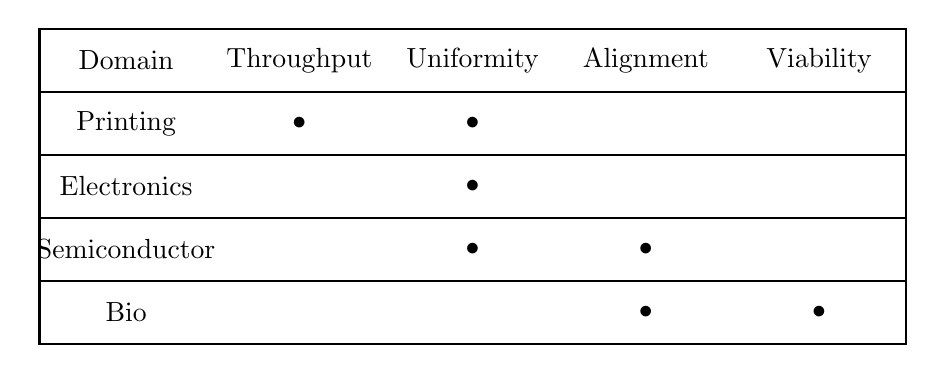
\begin{tikzpicture}
% Grid dimensions
\def\cw{22mm}\def\ch{8mm}
\def\x0{0}\def\y0{0}
% Headers
\draw[line] (\x0,\y0) rectangle ++(5*\cw,5*\ch);
\node at (\x0+0.5*\cw, \y0+4.5*\ch) {Domain};
\node at (\x0+1.5*\cw, \y0+4.5*\ch) {Throughput};
\node at (\x0+2.5*\cw, \y0+4.5*\ch) {Uniformity};
\node at (\x0+3.5*\cw, \y0+4.5*\ch) {Alignment};
\node at (\x0+4.5*\cw, \y0+4.5*\ch) {Viability};
% Rows
\def\row#1#2#3#4#5#6{
  \draw[line] (\x0,#2) rectangle ++(5*\cw,\ch);
  \node at (\x0+0.5*\cw,#2+0.5*\ch) {#1};
  \node at (\x0+1.5*\cw,#2+0.5*\ch) {#3};
  \node at (\x0+2.5*\cw,#2+0.5*\ch) {#4};
  \node at (\x0+3.5*\cw,#2+0.5*\ch) {#5};
  \node at (\x0+4.5*\cw,#2+0.5*\ch) {#6};
}
\row{Printing}{\y0+3*\ch}{$\bullet$}{$\bullet$}{}{}%
\row{Electronics}{\y0+2*\ch}{}{$\bullet$}{}{}%
\row{Semiconductor}{\y0+1*\ch}{}{$\bullet$}{$\bullet$}{}%
\row{Bio}{\y0+0*\ch}{}{}{$\bullet$}{$\bullet$}%
\end{tikzpicture}
\end{document}
